% schéma
\section{Kernel}
\begin{frame}
	\center{\huge{Noyau}}
	\begin{minipage}[t]{0.45\linewidth}
		\begin{figure}
			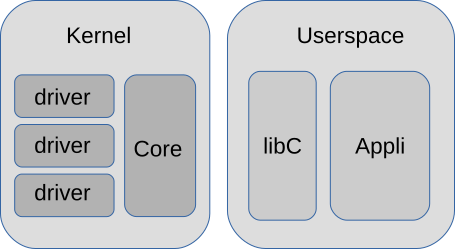
\includegraphics[height=5cm]{img/arch_linux_full.png}
			 \caption{kernel}
		\end{figure}
	\end{minipage}
	\begin{minipage}[t]{0.45\linewidth}
		\begin{itemize}
			\item Gère le matériel
			\item Gère les ressources
			\item Implémente certains protocoles
			\item Couche d'abstraction
			\item Isolé de l'espace utilisateur
			\item Composant critique
		\end{itemize}
	\end{minipage}

\end{frame}
\begin{frame}
	\center{\huge{Linux}}
	\begin{itemize}
		\item Beaucoup d'architectures
		\item Beaucoup de périphériques
		\item Beaucoup de fonctionnalités
		\item Communauté active
		\item Entièrement configurable
		\item Libre
		\item Documenté
		\item Polyvalent
	\end{itemize}
	\begin{block}{Variantes}
		\begin{itemize}
			\item Temps réeel : Preempt-RT, xenomai
			\item Microcontrolleur : uCLinux
			\item Sécurité : SELinux, grsecurity
		\end{itemize}
	\end{block}
\end{frame}
% choix de la version
\subsection{Drivers}
\begin{frame}
	\center{\huge{Drivers}}
	\begin{itemize}
		\item Support d'un périphérique
		\item Support d'un protocole
		\item Libre ou Propriétaire
	\end{itemize}
	\begin{block}{Kernel module}
		\item Extension du kernel
		\item Intégration statique ou dynamique
		\item Lié à une version du kernel
		\item Gestion des dépendances
	\end{block}
\end{frame}
% drivers, support
\subsection{Configuration}
\begin{frame}
		\begin{itemize}
			\item Choix des drivers
			\item Choix des fonctionnalités
			\item Options de debug
			\item Options d'optimisation
		\end{itemize}
	\begin{block}{Kconfig}
		\begin{itemize}
			\item Plusieurs UI
			\item Dépendances entre options
			\item Génère un fichier de conf
		\end{itemize}
	\end{block}

\end{frame}
% choix des options : selon matos, contraintes
